\documentclass[journal,12pt,twocolumn]{IEEEtran}
\usepackage{setspace}
\usepackage{gensymb}
\singlespacing
\usepackage[cmex10]{amsmath}
\usepackage{amsthm}
\usepackage{mathrsfs}
\usepackage{txfonts}
\usepackage{stfloats}
\usepackage{bm}
\usepackage{cite}
\usepackage{cases}
\usepackage{subfig}
\usepackage{longtable}
\usepackage{multirow}
\usepackage{enumitem}
\usepackage{mathtools}
\usepackage{steinmetz}
\usepackage{tikz}
\usepackage{circuitikz}
\usepackage{verbatim}
\usepackage{tfrupee}
\usepackage[breaklinks=true]{hyperref}
\usepackage{graphicx}
\usepackage{tkz-euclide}
\usetikzlibrary{calc,math}
\usepackage{listings}
\usepackage{color}                                            %%
\usepackage{array}                                            %%
\usepackage{longtable}                                        %%
\usepackage{calc}                                             %%
\usepackage{multirow}                                         %%
\usepackage{hhline}                                           %%
\usepackage{ifthen}                                           %%
\usepackage{lscape}     
\usepackage{multicol}
\usepackage{chngcntr}
\DeclareMathOperator*{\Res}{Res}
\renewcommand\thesection{\arabic{section}}
\renewcommand\thesubsection{\thesection.\arabic{subsection}}
\renewcommand\thesubsubsection{\thesubsection.\arabic{subsubsection}}
\renewcommand\thesectiondis{\arabic{section}}
\renewcommand\thesubsectiondis{\thesectiondis.\arabic{subsection}}
\renewcommand\thesubsubsectiondis{\thesubsectiondis.\arabic{subsubsection}}
\hyphenation{op-tical net-works semi-conduc-tor}
\def\inputGnumericTable{}                                 %%
\lstset
{
%language=C,
frame=single, 
breaklines=true,
columns=fullflexible
}
\begin{document}
\newtheorem{theorem}{Theorem}[section]
\newtheorem{problem}{Problem}
\newtheorem{proposition}{Proposition}[section]
\newtheorem{lemma}{Lemma}[section]
\newtheorem{corollary}[theorem]{Corollary}
\newtheorem{example}{Example}[section]
\newtheorem{definition}[problem]{Definition}
\newcommand{\comb}[2]{{}^{#1}\mathrm{C}_{#2}}
\newcommand{\BEQA}{\begin{eqnarray}}
\newcommand{\EEQA}{\end{eqnarray}}
\newcommand{\define}{\stackrel{\triangle}{=}}
\bibliographystyle{IEEEtran}
\raggedbottom
\setlength{\parindent}{0pt}
\providecommand{\mbf}{\mathbf}
\providecommand{\pr}[1]{\ensuremath{\Pr\left(#1\right)}}
\providecommand{\qfunc}[1]{\ensuremath{Q\left(#1\right)}}
\providecommand{\sbrak}[1]{\ensuremath{{}\left[#1\right]}}
\providecommand{\lsbrak}[1]{\ensuremath{{}\left[#1\right.}}
\providecommand{\rsbrak}[1]{\ensuremath{{}\left.#1\right]}}
\providecommand{\brak}[1]{\ensuremath{\left(#1\right)}}
\providecommand{\lbrak}[1]{\ensuremath{\left(#1\right.}}
\providecommand{\rbrak}[1]{\ensuremath{\left.#1\right)}}
\providecommand{\cbrak}[1]{\ensuremath{\left\{#1\right\}}}
\providecommand{\lcbrak}[1]{\ensuremath{\left\{#1\right.}}
\providecommand{\rcbrak}[1]{\ensuremath{\left.#1\right\}}}
\theoremstyle{remark}
\newtheorem{rem}{Remark}
\newcommand{\sgn}{\mathop{\mathrm{sgn}}}
\providecommand{\abs}[1]{\vert#1\vert}
\providecommand{\res}[1]{\Res\displaylimits_{#1}} 
\providecommand{\norm}[1]{\lVert#1\rVert}
%\providecommand{\norm}[1]{\lVert#1\rVert}
\providecommand{\mtx}[1]{\mathbf{#1}}
\providecommand{\mean}[1]{E[#1]}
\providecommand{\fourier}{\overset{\mathcal{F}}{ \rightleftharpoons}}
\providecommand{\ztransform}{\overset{\mathcal{Z}}{ \rightleftharpoons}}
%\providecommand{\hilbert}{\overset{\mathcal{H}}{ \rightleftharpoons}}
\providecommand{\system}{\overset{\mathcal{H}}{ \longleftrightarrow}}
%\newcommand{\solution}[2]{\textbf{Solution:}{#1}}
\newcommand{\solution}{\noindent \textbf{Solution: }}
\newcommand{\cosec}{\,\text{cosec}\,}
\providecommand{\dec}[2]{\ensuremath{\overset{#1}{\underset{#2}{\gtrless}}}}
\newcommand{\myvec}[1]{\ensuremath{\begin{pmatrix}#1\end{pmatrix}}}
\newcommand{\mydet}[1]{\ensuremath{\begin{vmatrix}#1\end{vmatrix}}}
\numberwithin{equation}{subsection}
\makeatletter
\@addtoreset{figure}{problem}
\makeatother
\let\StandardTheFigure\thefigure
\let\vec\mathbf
\renewcommand{\thefigure}{\theproblem}
\def\putbox#1#2#3{\makebox[0in][l]{\makebox[#1][l]{}\raisebox{\baselineskip}[0in][0in]{\raisebox{#2}[0in][0in]{#3}}}}
\def\rightbox#1{\makebox[0in][r]{#1}}
\def\centbox#1{\makebox[0in]{#1}}
\def\topbox#1{\raisebox{-\baselineskip}[0in][0in]{#1}}
\def\midbox#1{\raisebox{-0.5\baselineskip}[0in][0in]{#1}}
\vspace{3cm}


\title{EE3900 Gate Assignment-4}
\author{V Rahul - AI20BTECH11030}
\maketitle
\newpage
\bigskip
\renewcommand{\thefigure}{\theenumi}
\renewcommand{\thetable}{\theenumi}
Download all python codes from 
\begin{lstlisting}
    https://github.com/vrahul02/EE3900/tree/main/Gate-Assignment-4/Codes
\end{lstlisting}
%
and latex-tikz codes from 
%
\begin{lstlisting}
    https://github.com/vrahul02/EE3900/tree/main/Gate-Assignment-4/Gate-Assignment-4.tex
\end{lstlisting}
\section*{Problem Gate EC-1998 Q.1.16}
The $z$-transform of the time function
$\sum_{k=0}^{\infty} \delta (n-k)$ is\\
\begin{enumerate}
    \item $\frac{z-1}{z}$
    \item $\frac{z}{(z-1)^2}$
    \item $\frac{z}{z-1}$
    \item $\frac{(z-1)^2}{z}$
\end{enumerate}
\section*{Solution}
\begin{definition}\label{def:z}
    The $z$-transform of a function is defined as
    \begin{align}
        x[n] &\ztransform X(z)\\
        X(z) &=\sum_{n=-\infty}^{\infty} x[n]z^{-n}
    \end{align}
\end{definition}
x(n)
\begin{align}
    =&\sum_{k=0}^{\infty} \delta (n-k)\\
    =&\:\delta (n)+\delta (n-1)+\delta (n-2)+...\\
    =&\:u(n)
\end{align}
where $u(n)$ denotes the unit-step function\\
\begin{definition}\label{def:u_n}
    The $u[n]$ function is defined as
    \begin{align}
        u[n] = 
        \begin{cases}
        1 & n\geq0\\
        0 & otherwise
        \end{cases}
    \end{align}
\end{definition}
Thus,
\begin{align}
    \mathcal{Z}(x(n))=\mathcal{Z}(u(n))
\end{align}
Using~\eqref{def:z} and~\eqref{def:u_n}
\begin{align}
    X(z)&=\sum_{n=-\infty}^{\infty} u[n]z^{-n}\\
    &=\sum_{n=0}^{\infty} ({z^{-1}})^n
\end{align}
Using the formula for the sum of an infinite GP, we get:
\begin{align}
    X(z)&=\frac{1}{1-z^{-1}},\, ROC=\abs{z^-1} < 1\\
    &=\frac{z}{z-1},\, ROC=\abs{z}>1
\end{align}
\begin{figure}[!ht]
    \centering
    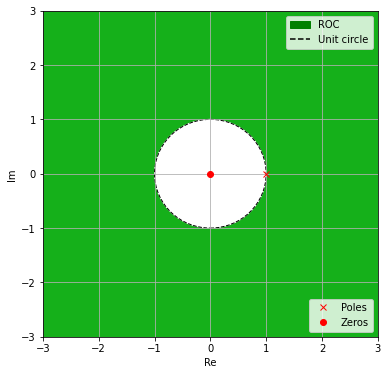
\includegraphics[width=\columnwidth]{Gate Assigment-4.png}
    \caption{Pole-zero plot of the system}
    \label{a}
\end{figure}
\begin{align}
    \mathcal{Z}(x(n))=\frac{z}{z-1}
\end{align}
Thus option 3) is correct
\end{document}